
\chapter{An Algorithm for the Computation of the
  Branches}\label{chap4}

IN\pageoriginale THIS CHAPTER, we describe an algorithm for finding
the local zero set of a mapping $f$ verifying the assumptions of Chapter
\ref{chap2}. When $f$ is {\em explicitly known}, we obtain an iterative
scheme with optimal rate of convergence. However, in the applications
to one paramenter problems in Banach spaces (such as those described
in Chapter \ref{chap3} for instance) $f$ is the reduced mapping which is
known {\em only theoretically}, because the mapping
$\widetilde{\varphi}$ coming from the Lyapunov-Schmidt reduction
(cf. Chapter \ref{chap1}, $\S 2$) involved in the definition of $f$ is
found through the {\em implict function theorem}.

What is explicitly available in this case is only a sequence
$(f_{\ell})$ of mappings tending to $f$ in some appropriate way and the
algorithm must be modified accordingly. Again, optimal rate of
convergence can be established but the proof is more delicate. For the
sake of brevity, we shall only outline the technical differences which
occur. The exposition follows Rabier-E1-Hajji \cite{33}. Full details can
be found in Appendix 2. This chapter is completed by an explicit
description of the algorithm in the case of problems of bifurcation
from the trivial branch. A comparison with the classical {\em
  ``Lyapunov-Schmidt method''} is given as a conclusion.

\section{A Short Review of the Method of Chapter
  II.}\label{chap4-sec1}

In\pageoriginale Chapter \ref{chap2}, we considered the problem of
finding the local zero set of a mapping $f$ of class $C^{m}, m \geq 1$,
from $\mathbb{R}^{n+1}$ into $\mathbb{R}^{n}$ (recall that it is not
restrictive to assume that $f$ is defined everywhere) satisfying the
following condition: There is an integer $1 \leq k \leq m$ such that
$$
D^{j}f(0) = 0 \quad 0 \leq j \leq k-1,
$$
and the mapping
$$
\widetilde{\xi} \epsilon \mathbb{R}^{n+1} \to q(\widetilde{\xi}) =
D^{k}f(0) \cdot (\widetilde{\xi})^{k} \epsilon \mathbb{R}^{n},
$$
verifies the condition $(\mathbb{R}-N.D.)$. Under this assumption, the
set 
$$
\{\widetilde{\xi} \epsilon S_{n} ; q(\widetilde{\xi}) = 0\}
$$
is finite and consists of the $2 \nu$ elements
$\widetilde{\xi}_{0}^{j}$, $1 \leq j \leq 2\nu$. Of course, as the
origin is an isolated solutioon of the equation $f(\widetilde{x}) = 0$
when $\nu = 0$, it is not restrictive to limit ourselves to the case
$\nu \geq 1$ for defining the algorithm. This assumption will be
implicitly made through-out this chapter.

Setting, for $(t, \widetilde{\xi}) \epsilon \mathbb{R} \times \mathbb{R}^{n+1}$
\begin{align*}
g(t, \widetilde{\xi}) & = \frac{k!}{t^{k}} f(t \widetilde{\xi}) \text{
if } t \neq 0,\\
g(0, \widetilde{\xi}) & = q(\widetilde{\xi}),
\end{align*}
it was observed for $r > 0$ that finding the solution $\widetilde{x}$
of the equation $f(\widetilde{x}) = 0$ with $0 < ||\widetilde{x}|| = t
< r$ was equivalent to finding $\widetilde{x}$\pageoriginale of the
form $\widetilde{x} = t\widetilde{\xi}$ where
\begin{align*}
& 0 < |t| < r, \widetilde{\xi} \epsilon S_{n},\\
& g(t, \widetilde{\xi}) = 0.
\end{align*}

Next, an essential step consisted in proving for $r > 0$ small enough
that the above equation was equivalent to solving the problem
\begin{align*}
& 0 < |t| < r, \widetilde{\xi} \epsilon \bigcup\limits_{j=1}^{2\nu}
  \sigma_{j},\\
& g(t, \widetilde{\xi}) = 0,
\end{align*}
where, for each $1 \leq j \leq 2\nu$, $\sigma_{j}$ denotes an {\em
  arbitrary} neighbourhood of $\widetilde{\xi}_{0}^{j}$ in
$S_{n}$. Taking the $\sigma_{j}$'s disjoint, the problem reduces to
the study of $2\nu$ {\em independent equations}
\begin{align*}
& 0 < |t| < r, \widetilde{\xi} \epsilon \sigma_{j},\\
& g(t, \widetilde{\xi}) = 0,
\end{align*}
for $1 \leq j \leq 2\nu$ where actually, $\nu$ of them (properly
selected) are sufficient, to provide all the other $\nu$ solutions
because of symmetry properties. From a practical point of view, it
remains to solve the equation $g(t, \widetilde{\xi}) = 0$ for $|t|$
small enough and $\widetilde{\xi} \epsilon S_{n}$ around one of the
points $\widetilde{\xi}_{0}^{j}$.

\section[Equivalence of Each Equation with a...]{Equivalence of Each
  Equation with a Fixed\hfil\break Point 
  Problem.}\label{chp4-sec2}

Since the specific value of the index $j$ is not important, we shall
denote any one of the points $\widetilde{\xi}_{0}^{j}$ by
$\widetilde{\xi}_{0}$. Given $\delta > 0$, we call\pageoriginale
$\triangle$ the closed ball in $\mathbb{R}^{n+1}$ with centre
$\widetilde{\xi}_{0}$ and radius $\delta / 2$. The {\em diameter}
$\delta$ of the ball $\triangle$ is always suppposed to satisfy the
condition
\begin{equation*}
0 < \delta < 1.\tag{2.1}\label{chap4-eq2.1}
\end{equation*}

Finally, we denote by $C$ the spherical cap centered at
$\widetilde{\xi}_{0}$ (playing the role of the negihbourhood
$\sigma_{j}$) defined by
\begin{equation*}
C = \triangle \cap S_{n}\tag{2.2}\label{chap4-eq2.2}
\end{equation*}
\begin{figure}[H]
\centering
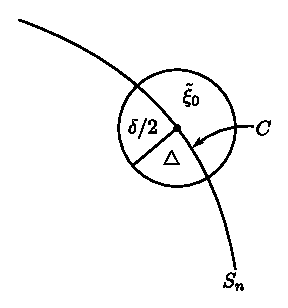
\includegraphics{figure/fig76-2.1_1.eps}
\caption{}
\end{figure}


We now establish two simple but crucial geometric properties. As in
Chapter \ref{chap2}, $||\cdot||$ denotes the euclidean norm.

\begin{lemma}\label{chap4-lem2.1}
(i) For every $\widetilde{\xi} \epsilon \triangle$, every
  $\widetilde{\zeta} \epsilon C$ and every $\widetilde{\tau} \epsilon
  T_{\widetilde{\zeta}} S_{n}$, one has
$$
|\widetilde{\xi} - \widetilde{\tau}| \geq 1 - \delta > 0.
$$

(ii) For\pageoriginale every $\widetilde{\xi} \epsilon C$ and every
$\widetilde{\zeta} \epsilon C$, one has
$$
\mathbb{R}^{n+1} = \mathbb{R} \widetilde{\xi} \oplus T_{\widetilde{\zeta}}S_{n}.
$$
\end{lemma}

\begin{proof}
Recall first, for $\widetilde{\zeta} \epsilon S_{n}$, that
$$
T_{\widetilde{\zeta}}S_{n} = \{\widetilde{\zeta}\}^{\perp}.
$$
To prove (i), we begin by writing
$$
||\widetilde{\xi} - \widetilde{\tau}|| \geq ||\widetilde{\zeta} -
\widetilde{\tau}|| - ||\widetilde{\xi} - \widetilde{\zeta}||
$$

Now, since $\widetilde{\zeta}$ and $\widetilde{\tau}$ are orthogonal
and $\widetilde{\zeta} \epsilon C \subset S_{n}$, we have
$$
||\widetilde{\zeta} - \widetilde{\tau}||^{2} =
||\widetilde{\zeta}||^{2} + ||\widetilde{\tau}||^{2} = 1 + ||\widetilde{\tau}||^{2}.
$$

Thus, as $\delta < 1$
$$
||\widetilde{\xi} - \widetilde{\tau}|| > 1 - ||\widetilde{\xi} -
\widetilde{\zeta}|| \geq 1 - \delta > 0.
$$

Next, to prove (ii), it suffices to show that
$\mathbb{R}\widetilde{\xi} \cap  T_{\widetilde{\zeta}}S_{n} = \{0\}$, namely
that $\widetilde{\xi} \notin T_{\widetilde{\zeta}}S_{n} =
\{\widetilde{\zeta}\}^{\perp}$. But a simple calulation shows that
$\widetilde{\xi} \epsilon C$ and $\widetilde{\zeta} \epsilon C$ are
never orthogonal where
$$
\delta < 2\sqrt{2 - \sqrt{2}}
$$
and hence when $\delta < 1$.

Since the mapping $q$ satisfies the condition $(\mathbb{R}-N.D.)$ and
$\widetilde{\xi}_{0}$ is one of the points $\widetilde{\xi}_{0}^{j}$,
we know that
$$
Dq(\widetilde{\xi}_{0}) |_{T_{\widetilde{\xi}_{0}} S_{n}} \epsilon
Isom (T_{\widetilde{\xi}_{0}}S_{n}, \mathbb{R}^{n}).
$$
\end{proof}

\begin{lemma}\label{chap4-lem2.2}
After shrinking $\delta > 0$ if necessary, one has
$$
Dq(\widetilde{\xi}) |_{T_{\widetilde{\xi}} S_{n}} \epsilon Isom
(T_{\widetilde{\xi}}S_{n}, \mathbb{R}^{n}),
$$\pageoriginale
for every $\widetilde{\xi} \epsilon C$. Besides, setting
\begin{equation*}
A(\widetilde{\xi}) = (Dq(\widetilde{\xi})
|_{T_{\widetilde{\xi}}S_{n}})^{-1} \epsilon \mathscr{L}
(\mathbb{R}^{n}, T_{\widetilde{\xi} S_{n}}) \subset
\mathscr{L}(\mathbb{R}^{n}, \mathbb{R}^{n+1}),\tag{2.3}\label{chap4-eq2.3}
\end{equation*}
one has
$$
A \epsilon C^{0} (C, \mathscr{L}(\mathbb{R}^{n}, \mathbb{R}^{n+1})).
$$
\end{lemma}

\begin{proof}
Let $B_{1}$ be the open unit ball in $\mathbb{R}^{n}$
$$
B_{1} = \{\widetilde{\xi}' \epsilon \mathbb{R}^{n} ;
||\widetilde{\xi}'|| < 1\}.
$$

By identifying $\mathbb{R}^{n+1}$ with the product $\mathbb{R}^{n}
\times \mathbb{R}\widetilde{\xi}_{0}$, the spherical cap $C$ is
homeomorphic to the closed ball $\overline{B}_{d/2} \subset
\mathbb{R}^{n}$ centred at the origin with diameter
$$
d = \delta \left(1 - \frac{\delta^{2}}{16}\right)^{\frac{1}{2}} < 1.
$$ 

This homeomorophism is induced by a $C^{\infty}$ -mapping
$$
\widetilde{\xi}' \epsilon B_{1} \to \theta(\widetilde{\xi}') =
(\widetilde{\xi}', (1 -
||\widetilde{\xi}'||^{2})^{\frac{1}{2}}\widetilde{\xi}_{0}) \epsilon
\mathbb{R}^{n+1} 
$$

It is immediately checked that
\begin{equation*}
D\theta(\widetilde{\xi}') \epsilon Isom (\mathbb{R}^{n},
T_{\theta(\widetilde{\xi}')}S_{n}) \subset \mathscr{L}
(\mathbb{R}^{n}, \mathbb{R}^{n+1}),\tag{2.4}\label{chap4-eq2.4}
\end{equation*}
for every $\widetilde{\xi}' \epsilon B_{1}$.

The mapping $q \bullet \theta$ is of class $C^{\infty}$ from $B_{1}$
into $\mathbb{R}^{n}$ and by differentiating
$$
D(q \bullet \theta) (\widetilde{\xi}') = Dq(\theta(\widetilde{\xi}'))
\cdot D\theta(\widetilde{\xi}').
$$

Since\pageoriginale the mapping $D\theta(\widetilde{\xi}')$ takes its
values in the space $T_{\theta(\widetilde{\xi}')} S_{n}$, this can be
rewritten as
\begin{equation*}
D(q \bullet \theta)(\widetilde{\xi}') = Dq(\theta(\widetilde{\xi}'))
|_{T_{\theta}(\widetilde{\xi}') S_{n}} \cdot
D\theta(\widetilde{\xi}').\tag{2.5}\label{chap4-eq2.5} 
\end{equation*}

In particular, for $\widetilde{\xi}' = 0$
$$
D(q \bullet \theta)(0) = Dq(\widetilde{\xi}_{0})
|_{T_{\widetilde{\xi}_{0}} S_{n}} \cdot D\theta(0).
$$

As $Dq(\widetilde{\xi}_0) |_{T_{\widetilde{\xi}_{0}} S_{n}} \epsilon
Isom (T_{\widetilde{\xi}_{0}} S_{n}, \mathbb{R}^{n})$ and $D\theta(0)
\epsilon Isom (\mathbb{R}^{n}, T_{\widetilde{\xi}_{0}} S_{n})$, we
deduce
$$
D(q \bullet \theta)(0) \epsilon Isom (\mathbb{R})^{n}.
$$

By continuity, we may assume that $d > 0$ (or, equivalently, $\delta >
0$) has been chosen small enough for $D(q \bullet \theta)
(\widetilde{\xi}')$ to be an isomorphism for every $\widetilde{\xi}'
\epsilon \overline{B}_{d/2}$. Together with (\ref{chap4-eq2.4}),
relation (\ref{chap4-eq2.5}) shows that
\begin{equation*}
Dq(\theta(\widetilde{\xi}')) |_{T_{\theta(\widetilde{\xi}')S_{n}}} =
D(q \bullet \theta) (\widetilde{\xi}') \cdot
[D\theta(\widetilde{\xi}')]^{-1} \epsilon Isom
(T_{\theta(\widetilde{\xi}')}S_{n}, \mathbb{R}^{n}).\tag{2.6}\label{chap4-eq2.6}
\end{equation*}

Hence
$$
Dq(\widetilde{\xi}) |_{T_{\widetilde{\xi}}S_{n}} \epsilon Isom
(T_{\widetilde{\xi}} S_{n}, \mathbb{R}^{n}),
$$
for every $\widetilde{\xi} \epsilon C$ since $\theta$ is a bijection
from $\overline{B}_{d/2}$ to $C$. Now, taking the inverse in
(\ref{chap4-eq2.6}) and according to the definition of $A$ in
(\ref{chap4-eq2.3}), we get
$$
A(\theta(\widetilde{\xi}')) = [Dq(\theta(\widetilde{\xi}'))
  |_{T_{\theta(\widetilde{\xi}')}S_{n}}]^{-1} =
D\theta(\widetilde{\xi}') \cdot (D(q \bullet \theta) (\widetilde{\xi}'))^{-1}.
$$
 
The continuity of the mappings $D_{\theta}$ (with values in
$\mathscr{L}(\mathbb{R}^{n}, \mathbb{R}^{n+1})$) and $D(q \bullet
\theta)$\pageoriginale (with values in Isom $(\mathbb{R}^{n})$) and
the continuity of the mapping $L \to L^{-1}$ in teh set Isom
$(\mathbb{R}^{n})$ shows that the mapping $A \bullet \theta$ is
continuous on the ball $\overline{B}_{d/2}$. The continuity of $A$
follows since $\theta$ is a homeomorphisn between $\overline{B}_{d/2}$
and $C$.
\end{proof}

\begin{remark}\label{chap4-rem2.1}
With an obvious modification of the above arguments, we see that the
mapping $A \bullet \theta$ is actually $C^{\infty}$ around the origin
of $\mathbb{R}^{n}$. As $\theta^{-1}$ is a chart of the sphere $S_{n}$
centered at the point $\widetilde{\xi}_{0}$, this means that $A$ is of class
$C^{\infty}$ on a neighbourhood of $\widetilde{\xi}_{0}$ in the sphere
$S_{n}$. More generally, replacing the mapping $q(\widetilde{\xi})$ by
$q(t, \widetilde{\xi})$ a similar proof shows that the mapping
$$
(t, \widetilde{\xi}) \to [D_{\widetilde{\xi}}g (t, \widetilde{\xi}) |_{T_{\widetilde{\xi}}S_{n}}]^{-1}
$$
is of class $C^{\ell}$ in a neighbourhood of $(0,
\widetilde{\xi}_{0})$ in $\mathbb{R} \times S_{n}$ whenever
$D_{\widetilde{\xi}}g$ is of class $C^{\ell}$. This result was used in
the proof of Theorem \ref{chap2-thm4.1} of Chapter \ref{chap2} (with
$\ell = m-k$).
\end{remark}

Let us now fix $0 < \delta < 1$ such that Lemma \ref{chap4-lem2.2}
holds. Given a triple $(t, \widetilde{\zeta}_{0}, \widetilde{\xi})
\epsilon \mathbb{R} \times C \times \triangle$, the mapping
\begin{equation*}
M(t, \widetilde{\zeta}_{0}, \widetilde{\xi}) = \widetilde{\xi} -
A(\widetilde{\zeta}_{0}) \cdot g(t, \widetilde{\xi}) \epsilon \mathbb{R}^{n+1},\tag{2.7}\label{chap4-eq2.7}
\end{equation*}
is well-defined ane we have (recalling that $g(0, \widetilde{\xi}_{0})
= q(\widetilde{\xi}_{0}) = 0$)
\begin{equation*}
M(0, \widetilde{\zeta}_{0}, \widetilde{\xi}_{0}) = \widetilde{\xi}_{0}.\tag{2.8}\label{chap4-eq2.8}
\end{equation*}

Taking $\widetilde{\zeta} = \widetilde{\zeta}_{0}$ and
$\widetilde{\tau} = A(\widetilde{\zeta}_{0}) \cdot g(t, \xi)$ in Lemma
\ref{chap4-lem2.1}(i), we get
$$
||M(t, \widetilde{\zeta}_{0}, \widetilde{\xi})|| \geq 1 - \delta > 0.
$$

Thus,\pageoriginale the mapping
\begin{equation*}
N(t, \widetilde{\zeta}_{0}, \widetilde{\xi}) = \frac{M(t,
  \widetilde{\zeta}_{0}, \widetilde{\xi})}{||M(t,
  \widetilde{\zeta}_{0}, \widetilde{\xi})||} \epsilon S_{n},\tag{2.9}\label{chap4-eq2.9}
\end{equation*}
is well-defined in $\mathbb{R} \times C \times \triangle$ and 
\begin{equation*}
N(0, \widetilde{\zeta}_{0}, \widetilde{\xi}_{0}) = \widetilde{\xi}_{0}.\tag{2.10}\label{chap4-eq2.10}
\end{equation*}

\begin{theorem}\label{chap4-thm2.1}
Let $(t, \widetilde{\zeta}_{0}) \epsilon \mathbb{R} \times C$ be given.
\begin{enumerate}
\item[(i)] Let $\widetilde{\xi} \epsilon C$ be such that $g(t,
  \widetilde{\xi}) = 0$. Then $\widetilde{\xi}$ is a fixed point of
  the mapping $N(t, \widetilde{\zeta}_{0}, \cdot)$

\item[(ii)] Conversely, let $\widetilde{\xi} \epsilon \triangle$ be a
  fixed point of the mapping $N(t, \widetilde{\zeta}_{0},
  \cdot)$. Then, $\widetilde{\xi} \epsilon C$ and $g(t,
  \widetilde{\xi}) = 0$.
\end{enumerate}
\end{theorem}

\begin{proof}
Part (i) is obvious since, for $\widetilde{\xi} \epsilon C$ such that
$g(t, \widetilde{\xi}) = 0$ one has $N(t, \widetilde{\zeta}_{0},
\widetilde{\xi}) = \widetilde{\xi} / ||\widetilde{\xi}|| =
\widetilde{\xi}$. Conversely, the mapping $N(t, \widetilde{\zeta}_{0},
\cdot)$ takes its values in $S_{n}$ so that any fixed point
$\widetilde{\xi} \epsilon \triangle$ of the mapping $N(t,
\widetilde{\zeta}_{0}, \cdot)$ must belong to $\triangle \cap S_{n} =
C$. Next, the relation $N(t, \widetilde{\zeta}_{0}, \widetilde{\xi}) =
\widetilde{\xi}$ also becomes
$$
\widetilde{\xi}(1 - ||\widetilde{\xi} - A(\widetilde{\zeta}_{0}) \cdot
g(t, \widetilde{\xi})||) = A(\widetilde{\xi}_{0}) \cdot g(t, \widetilde{\xi}).
$$

But the left hand side is collinear with $\widetilde{\xi}$, while the
right hand side belongs to the space
$T_{\widetilde{\zeta}_{0}}S_{n}$. By lemma \ref{chap4-lem2.1}(ii),
both sides must vanish. In prticular, $A(\widetilde{\zeta_{0}}) \cdot
g(t, \widetilde{\xi}) = 0$ and hence $g(t, \widetilde{\xi}) = 0$ since
the linear operator $A(\widetilde{\zeta}_{0})$ is one-to-one.
\end{proof}

\begin{remark}\label{chap4-rem2.2}
As announced, the problem reduces to finding the fixed points of a
given mapping. We emphasize that it is essential, in practice,
that\pageoriginale the vector $\widetilde{\zeta}_{0}$ be allowed to be
arbitrary in  $C$. Indeed, the ``natural'' choice $\widetilde{\zeta}_{0} =
\widetilde{\xi}_{0}$ is {\em not realistic} in the applications
beacuse $\widetilde{\xi}_{0}$ {\em is not known} exactly in general.
\end{remark}

\section{Convergence of the Successive Approximation
  Method.}\label{chap4-sec3}

From Theorem \ref{chap4-thm2.1}, a constructive method for finding the
solutions of the equation $g(t, \widetilde{\xi}) = 0$ in $\mathbb{R}
\times C$ consists in applying the successive approximation method to
the mapping
\begin{equation*}
\widetilde{\xi} \epsilon \triangle \to N(t, \widetilde{\zeta}_{0},
\widetilde{\xi}) \epsilon C,\tag{3.1}\label{chap4-eq3.1}
\end{equation*}
where $\widetilde{\zeta}_{0} \epsilon C$ is arbitrarily fixed. In what
follows, we prove after shrinking $\delta$ if necessary that there is
$r > 0$ such that the mapping (\ref{chap4-eq3.1}) is a {\em
  contraction} of $\triangle$ into itself for every pair $(t,
\widetilde{\zeta}) \epsilon (-r, r) \times C$.

As a preliminary step, let us observe, by the continuity of the
mapping $A$ (Lemma \ref{chap4-lem2.2}) and by the continuity of $g$ and
$D_{\widetilde{\xi}}g$ on $\mathbb{R} \times \mathbb{R}^{n+1}$
(cf. Chapter \ref{chap2}, Lemma \ref{chap2-lem3.3}), that the mapping
$M$ is continuous on $\mathbb{R} \times C \times \triangle$ and its
partial derivative $D_{\widetilde{\xi}}M$ exists and is continuous on
$\mathbb{R} \times C \times \triangle$. More precisely, for every
$\widetilde{h} \epsilon \mathbb{R}^{n+1}$, 
$$
D_{\widetilde{\xi}}M(t, \widetilde{\zeta}_{0}, \widetilde{\xi}) \cdot
\widetilde{h} = \widetilde{h} - A(\widetilde{\zeta}_{0}) \cdot
D_{\widetilde{\xi}}g(t, \widetilde{\xi}) \cdot \widetilde{h}.
$$

In particular, with $(t, \widetilde{\zeta}_{0}, \widetilde{\xi}) = (0,
\widetilde{\xi}_{0}, \widetilde{\xi}_{0})$ we find:
\begin{equation*}
D_{\widetilde{\xi}}M(t, \widetilde{\xi}_{0}, \widetilde{\xi}_{0})
\cdot \widetilde{h} = \widetilde{h} - A(\widetilde{\xi}_{0}) \cdot
D_{\widetilde{\xi}}g(0, \widetilde{\xi}_{0}) \cdot \widetilde{h}.\tag{3.2}\label{chap4-eq3.2}
\end{equation*}

But $D_{\widetilde{\xi}}g(0, \widetilde{\xi}_{0}) =
Dg(\widetilde{\xi}_{0})$ and by definition of $A$, it follows that
$$
D_{\widetilde{\xi}}M(0, \widetilde{\xi}_{0}, \widetilde{\xi}_{0})
|_{T_{\widetilde{\xi}_{0}}S_{n}} = 0.
$$\pageoriginale

Next, taking $\widetilde{h} = \widetilde{\xi}_{0}$ in
(\ref{chap4-eq3.2}) we find
$$
D_{\widetilde{\xi}}M(0, \widetilde{\xi}_{0} ; \widetilde{\xi}_{0})
\cdot \widetilde{\xi}_{0} = \widetilde{\xi}_{0} -
A(\widetilde{\xi}_{0}) \cdot D_{\widetilde{\xi}}q(0,
\widetilde{\xi}_{0}) \cdot \widetilde{\xi}_{0} = \widetilde{\xi}_{0},
$$
because $D_{\widetilde{\xi}}q(0, \widetilde{\xi}_{0}) =
kq(\widetilde{\xi}_{0}) = 0$. The space $\mathbb{R}^{n+1}$ being the
orthogonal direct sum of the spaces $\mathbb{R}\widetilde{\xi}_{0}$
and $T_{\widetilde{\xi}_{0}}S_{n}$, these relations mean that the
partial dericative $D_{\widetilde{\xi}}M(0, \widetilde{\xi}_{0},
\widetilde{\xi}_{0})$ is nothing but the {\em orthogonal projection}
onto the space $\mathbb{R}\widetilde{\xi}_{0}$, namely
$$
D_{\widetilde{\xi}}M(0, \widetilde{\xi}_{0}, \widetilde{\xi}_{0})
\cdot \widetilde{h} = (\widetilde{\xi}_{0} | \widetilde{h})\widetilde{\xi}_{0},
$$
for every $\widetilde{h} \epsilon \mathbb{R}^{n+1}$ where $(\cdot |
\cdot)$ denotes the canonical inner product of $\mathbb{R}^{n+1}$.

As a result, the mapping $N$ is continuous on $\mathbb{R} \times C
\times \triangle$ and its partial derivative $D_{\widetilde{\xi}}N$
exists and is continuous on $\mathbb{R} \times C \times \triangle$. We
now proceed to show that
$$
D_{\widetilde{\xi}}N(0, \widetilde{\xi}_{0}, \widetilde{\xi}_{0}) = 0.
$$

An elementary computation provides
{\fontsize{10}{12}\selectfont
$$
D_{\widetilde{\xi}}N(t, \widetilde{\zeta}_{0}, \widetilde{\xi}) \cdot
\widetilde{h} = \frac{D_{\widetilde{\xi}}M(t, \widetilde{\zeta}_{0},
  \widetilde{\xi})\cdot \widetilde{h}}{||M(t, \widetilde{\zeta}_{0},
  \widetilde{\xi})||} - \frac{(D_{\widetilde{\xi}}M(t,
  \widetilde{\zeta}_{0}, \widetilde{\xi})\cdot \widetilde{h} |M(t,
  \widetilde{\zeta}_{0}, \widetilde{\xi}))}{||M(t,
  \widetilde{\zeta}_{0}, \widetilde{\xi})||^{3}} M(t,
\widetilde{\zeta}_{0}, \widetilde{\xi}).
$$}
With $(t, \widetilde{\zeta}_{0}, \widetilde{\xi}) = (0,
\widetilde{\xi}_{0}, \widetilde{\xi}_{0})$ and since $M(0,
\widetilde{\xi}_{0}, \widetilde{\xi}_{0}) = \widetilde{\xi}_{0}$ and
$D_{\widetilde{\xi}}M(0,\break \widetilde{\xi}_{0}, \widetilde{\xi}_{0})
\cdot \widetilde{h} = (\widetilde{\xi}_{0} | \widetilde{h})$, we get
$$
D_{\widetilde{\xi}}N(t, \widetilde{\zeta}_{0}, \widetilde{\xi}) \cdot
\widetilde{h} = (\widetilde{\xi}_{0} |
\widetilde{h})\widetilde{\xi}_{0} - ((\widetilde{\xi}_{0} |
\widetilde{h})\widetilde{\xi}_{0} | \widetilde{\xi}_{0}) = 0.
$$

\begin{theorem}\label{chap4-thm3.1}
Let\pageoriginale $0 < \gamma < 1$ be a given constant. After shrinking $\delta > 0$ if necessary, there exists $r > 0$ such that the mapping $N(t, \widetilde{\zeta}, \cdot)$ is Lipschitz-continuous with constant $\gamma$ from the ball $\triangle$ into itself for every pair $(t, \widetilde{\zeta}) \epsilon [-r, r] \times C$.  
\end{theorem}

\begin{proof}
From the relation $D_{\widetilde{\xi}}N(0, \widetilde{\xi}_{0},
\widetilde{\xi}_{0}) = 0$ and the continuity of $D_{\widetilde{\xi}}N$
in $\mathbb{R} \times C \times \triangle$, we deduce that there is a
neighbourhood of $(0, \widetilde{\xi}_{0}, \widetilde{\xi}_{0})$ in
$\mathbb{R} \times S_{n} \times \mathbb{R}^{n+1}$ in which
$||D_{\widetilde{\xi}}N(t, \widetilde{\zeta}_{0}, \widetilde{\xi})||$
is bounded by $\gamma$. Clearly, after shrinking $\delta$ (hence
$\triangle$ and $C$ simultaneously), the neighbourhood in question can
be taken as the product $[-r, r] \times C \times \triangle$ for $r >
0$ small enough. Hence, by Taylor's formula (since $\triangle$ is
convex)
$$
||N(t, \widetilde{\zeta}_{0}, \widetilde{\xi}) - N(t,
\widetilde{\zeta}_{0}, \widetilde{\zeta})|| < \gamma||\widetilde{\xi}
- \widetilde{\zeta}||
$$
for every $(t, \widetilde{\zeta}_{0}) \epsilon [-r, r] \times C$ and
every $\widetilde{\xi}, \widetilde{\zeta} \epsilon \triangle$. In
other words, for every $(t, \widetilde{\zeta}_{0}) \epsilon [-r, r]
\times C$, the mapping $N(t, \widetilde{\zeta}, \cdot)$ is
Lipschitz-continuous with constant $\gamma$ in the ball
$\triangle$. The property is obviously not affected by {\em
  arbitrarily shrinking} $r > 0$. Let us then {\em fix} $\delta$ as
above, which determines the ball $\triangle$ and the spherical cap
$C$. We shall complete the proof by showing, for $r > 0$ small enough,
that the mapping $N(t, \widetilde{\xi}_{0}, \cdot)$ maps the ball $\triangle$ into
itself for every point $(t, \widetilde{\zeta}_{0}) \epsilon [-r, r]
\times C$. Indeed, for $\widetilde{\xi} \epsilon \triangle$ and since
$N(0, \widetilde{\zeta}_{0}, \widetilde{\xi}_{0}) =
\widetilde{\xi}_{0}$ for every $\widetilde{\zeta}_{0} \epsilon C$
(cf. (\ref{chap4-eq2.10})), one has
\begin{align*}
||N(t, \widetilde{\zeta}_{0}, \widetilde{\xi}) & -
\widetilde{\xi}_{0}|| = ||N(t, \widetilde{\zeta}_{0}, \widetilde{\xi})
- N(0, \widetilde{\zeta}_{0}, \widetilde{\xi}_{0})|| \leq\\
\leq ||N(t, \widetilde{\zeta}_{0}, \widetilde{\xi}) & - N(t,
\widetilde{\zeta}_{0}, \widetilde{\xi}_{0})|| + ||N(t,
\widetilde{\zeta}_{0}, \widetilde{\xi}_{0}) - N(0,
\widetilde{\zeta}_{0}, \widetilde{\xi}_{0})||.
\end{align*}

The\pageoriginale first term is bounded by $\gamma||\widetilde{\xi} -
\widetilde{\xi}_{0}||$, thus by $\gamma \delta / 2$. Finally, due to
the {\em uniform continuity} of the function $N(\cdot, \cdot,
\widetilde{\xi}_{0})$ on compact sets, we deduce that $r > 0$ can be
chosen so that the second term is bounded by $(1 - \gamma) \delta/2$
and our assertion follows.
\end{proof} 

\section{Description of the Algorithm.}\label{chap4-sec4}

The algorithm of computation of the solutions of the equation $g(t,
\widetilde{\xi}) = 0$ in $[-r, r] \times C$ is immediate from Theorem
\ref{chap4-thm3.1} : fixing $t \epsilon [-r, r]$ and choosing an
arbitrary element $\widetilde{\xi}_{0} \epsilon C$, we define the
sequence $(\widetilde{\zeta}_{\ell})$ through the formula
\begin{equation*}
\widetilde{\zeta}_{\ell + 1} = N(t, \widetilde{\zeta}_{0},
\widetilde{\zeta}_{\ell}), \ell \geq 0.\tag{4.1}\label{chap4-eq4.1}
\end{equation*}

This sequence tends to the unique fixed point $\widetilde{\xi}
\epsilon \triangle$ of the mapping $N(t, \widetilde{\zeta}_{0},
\cdot)$ which actually belongs to $C$ and is a solution of the equation
$g(t, \widetilde{\xi}) = 0$ (Theorem \ref{chap4-thm2.1}).

For $t \neq 0$, the sequence
$$
\widetilde{x}_{\ell} = t\widetilde{\zeta}_{\ell}
$$
tends to $\widetilde{x} = t\widetilde{\xi}$, one among the $2\nu$
solutions with euclidean norm $|t|$ of the equation $f(\widetilde{x}) =
0$. Of course, for $t = 0$, the sequence $(\widetilde{\zeta}_{\ell})$
tends to $\widetilde{\xi}_{0}$, unique solution in $C$ of the equation
$g(0, \widetilde{\xi})(= q(\widetilde{\xi})) = 0$.

\begin{remark}\label{chap4-rem4.1}
Incidentally, observe that the above algorithm allows to find
arbitrarily close approximations of $\widetilde{\xi}_{0}$ when only a
``rough'' estimate (i. e. $\widetilde{\zeta}_{0}$) of it is known.
\end{remark}

Since\pageoriginale our algorithm uses nothing but the contraction
mapping principle, the rate of convergence is {\em geometrical}. More precisely
$$
||\widetilde{\zeta}_{\ell} - \widetilde{\xi}|| < \gamma^{\ell}
||\widetilde{\zeta}_{0} - \widetilde{\xi}||,
$$
for every $\ell \geq 0$, where $0 < \gamma < 1$ is the constant
involved in Theorem \ref{chap4-thm3.1}. Thus as the points
$\widetilde{\zeta}_{0}$ and $\widetilde{\xi}$ belong to the ball
$\triangle$, one has $||\widetilde{\zeta}_{0} - \widetilde{\xi}|| <
\delta < 1$ and hence
$$
||\widetilde{\zeta}_{\ell} - \widetilde{\xi}|| \leq \gamma^{\ell}
\delta \leq \gamma^{\ell},
$$
for $\ell > 0$. Multiplying these inequalities by $|t|$, we get
\begin{equation*}
||\widetilde{x}_{\ell} - \widetilde{x}|| \leq \gamma^{\ell}
||\widetilde{x}_{0} - \widetilde{x}|| \leq |t| \gamma^{\ell},\tag{4.2}\label{chap4-eq4.2}
\end{equation*}
for $\ell \geq 0$.

Let us now make the scheme (\ref{chap4-eq4.1}) explicit. As
$$
g(t, \widetilde{\xi}) = \frac{k!}{t^{k}} f(t \widetilde{\xi}) \text{
  for } t \neq 0,
$$
and by the definition of the mapping $N$ in (\ref{chap4-eq2.9}), we get
\begin{equation*}
\begin{cases}
& \widetilde{\zeta}_{\ell + 1} =
  \frac{\widetilde{\zeta}_{\ell}}{||\widetilde{\zeta}_{\ell}||},\\
& \widetilde{\zeta}_{\ell} = \widetilde{\zeta}_{\ell} -
  \frac{k!}{t^{k}} A(\widetilde{\zeta}_{0}) \cdot f(t
  \widetilde{\zeta}_{\ell}), \ell \geq 0.
\end{cases}\tag{4.3}\label{chap4-eq4.3}
\end{equation*}

A scheme for the computation of the sequence $(\widetilde{x}_{\ell})$
can be immediately derived. Since $\widetilde{x}_{0} =
t\widetilde{\zeta}$, the iterate $\widetilde{x}_{\ell + 1} =
t\widetilde{\zeta}_{\ell + 1}$ is defined by 
\begin{equation*}
\begin{cases}
& \widetilde{x}_{\ell + 1} = |t|
  \frac{\widetilde{x}_{\ell}}{||\widetilde{x}_{\ell}||},\\
& \widetilde{x}_{\ell} = \widetilde{x}_{\ell} - \frac{k!}{t^{k-1}}
  A(\widetilde{\zeta}_{0}) \cdot f(\widetilde{x}_{\ell}), \ell \geq 0.
\end{cases}\tag{4.4}\label{chap4-eq4.4}
\end{equation*}

\begin{remark}\label{chap4-rem4.2}
When\pageoriginale $t = 0$, the sequence $(\widetilde{\zeta}_{\ell})$
is defined by
\begin{equation*}
\begin{cases}
& \widetilde{\zeta}_{\ell + 1} =
  \frac{\widetilde{\zeta}_{\ell}}{||\widetilde{\zeta}_{\ell}||},\\
& \widetilde{\zeta}_{\ell} = \widetilde{\zeta}_{\ell} -
  A(\widetilde{\zeta}_{0}) \cdot q(\widetilde{\zeta}_{\ell}), \ell
  \geq 0.
\end{cases}
\end{equation*}

Of course, the sequence $(\widetilde{x}_{\ell})$ is the constant one
$\widetilde{x}_{\ell} = 0$.
\end{remark}

\begin{remark}\label{chap4-rem4.3}
(Practical method): Note that the computation of the term 
$$
A(\widetilde{\zeta}_{0}) \cdot f(\widetilde{x}_{\ell}),
$$
does not require the explicit form of the linear operator
$A(\widetilde{\zeta}_{0})$. Indeed, by means of classical algorithm
for solving linear systems, it is obtained as the solution
$\widetilde{\tau} \epsilon T_{\widetilde{\zeta}_{0}} S_{n} =
\{\widetilde{\zeta}_{0}\}^{\perp}$ of the equation
\begin{equation*}
Dq(\widetilde{\zeta}_{0}) \cdot \widetilde{\tau} = f(\widetilde{x}_{\ell}).\tag{4.5}\label{chap4-eq4.5}
\end{equation*}

From the fact that the components of the mapping $q$ are polynomials and
hence are completely determined by a finite number of coefficients
(depending on the derivative $D^{k}f(0)$), the linear mapping
$Dq(\widetilde{\zeta}_{0})$ is completely determined by
$\widetilde{\zeta}_{0}$ and these coefficients. The tangent space
$T_{\widetilde{\zeta}}S_{n} = \{\widetilde{\zeta}_{0}\}^{\perp}$ also
is completely determined by $\widetilde{\zeta}_{0}$, which makes it
possible to solve the equation (\ref{chap4-eq4.5}) in practice.
\end{remark}

\begin{remark}\label{chap4-rem4.4}
The case $k = 1$ is the case when the Implicit function theorem
applies. The mapping $q$ is the linear mapping $Df(0)$ and the vector
$\widetilde{\xi}_{0}$ is a normalized vector of the one-dimensional
space $\Ker Df(0)$.\pageoriginale The sequence $(\widetilde{x}_{\ell})$
is defined by the simples relation (after choosing $\widetilde{x}_{0}
= t\widetilde{\zeta}_{0}$)
\begin{equation*}
\begin{cases}
& \widetilde{x}_{\ell + 1} = |t|
  \frac{\widetilde{x}_{\ell}}{||\widetilde{x}_{\ell}||},\\
& \widetilde{x}_{\ell} = \widetilde{x}_{\ell} - (Df(0)
  |_{\{\widetilde{\zeta}_{0}\}^{\perp}})^{-1} f(\widetilde{x}_{\ell}),
  \ell \geq 0,
\end{cases}
\end{equation*}
where $\widetilde{\zeta}_{0} \epsilon S_{n}$ is ``close enough'' to
$\widetilde{\xi}_{0}$. This sequence tends to one of the (two)
solutions with eucliden norm $|t|$ of the equation $f(\widetilde{x}) =
0$.
\end{remark}

\section[A Generalization to the Case.....]{A Generalization to the Case When the Mapping $f$ is not  Explicitly Known.}\label{chap4-sec5} 

For the reasons we explained at the beginning of this chapter, it is
important to extend the algorithm described in $\S 4$ to the case when
the mapping $f$ is not explicitly known but a sequence $(f_{\ell})$
tending to $f$ is available.

More precisely, the mapping $f$ verifying the same assumptions as
before, we shall assume that there is an open neighbourhood
$\mathscr{O}$ of the origin in $\mathbb{R}^{n+1}$ such that $f$ is the
limit of $(f_{\ell})$ {\em in the space}
$C^{k}(\overline{\mathscr{O}}, \mathbb{R}^{n})$ (equipped with its
usual Banach space structure). Besides, we shall assume
\begin{align*}
& D^{j}f_{\ell}(0) = 0, 0 \leq j \leq
  k-1,\tag{5.1}\label{chap4-eq5.1}\\
& D^{k}f_{\ell}(0) = D^{k}f(0),\tag{5.2}\label{chap4-eq5.2}
\end{align*}
so that {\em the first $k$ derivatives of} $f$ and $f_{\ell}$ at the
origin {\em coincide for every} $\ell \geq 0$.

\begin{remark}\label{chap4-rem5.1}
The\pageoriginale conditions (\ref{chap4-eq5.1})-(\ref{chap4-eq5.2})
may seem very restrictive.\break However, they are quite adapted to the
applications to one-parameter problems in Banch spaces, as we shall
see later on.
\end{remark}

If this is the case, the mapping
\begin{equation*}
\widetilde{\xi} \epsilon \mathbb{R}^{n+1} \to q(\widetilde{\xi}) =
D^{k}f(0) \cdot (\widetilde{\xi})^{k} \epsilon \mathbb{R}^{n},\tag{5.3}\label{chap4-eq5.3}
\end{equation*}
can as well be defined through any of the mappings $f_{\ell}$, namely
\begin{equation*}
q(\widetilde{\xi}) = D^{k}f_{\ell}(0) (\widetilde{\xi})^{k},\tag{5.4}\label{chap4-eq5.4}
\end{equation*}
for every $\ell \geq 0$. As usual, we shall assume that it verifies
the condition $(\mathbb{R}-N.D.)$.

In analogy with $\S\S 1$ and 2. let us define, for every $\ell \geq
0$,
\begin{align*}
& g_{\ell}(t, \widetilde{\xi}) = \frac{k!}{t^{k}}f_{\ell}
  (t\widetilde{\xi}) \text{ for } t \neq
  0,\tag{5.5}\label{chap4-eq5.5}\\
& g_{\ell}(0, \widetilde{\xi}) = q(\widetilde{\xi}),\tag{5.6}\label{chap4-eq5.6}\\
& M_{\ell}(t, \widetilde{\zeta}_{0}, \widetilde{\xi}) =
  \widetilde{\xi} - A(\widetilde{\zeta}_{0}) \cdot g_{\ell} (t,
  \widetilde{\xi}),\tag{5.7}\label{chap4-eq5.7}\\
& N_{\ell}(t, \widetilde{\zeta}_{0}, \widetilde{\xi}) =
  \frac{M_{\ell}(t, \widetilde{\zeta}_{0},
    \widetilde{\xi})}{||M_{\ell}(t, \widetilde{\zeta}_{0}, \widetilde{\xi})||}.\tag{5.8}\label{chap4-eq5.8}
\end{align*}

Of course, the key point is that a {\em uniform choice} of $0 < \delta
< 1$ can be made for defining the mapping $M_{\ell}$ and $N_{\ell}$ in
(\ref{chap4-eq5.7})-(\ref{chap4-eq5.8}) because the way of shrinking
$\delta$ in $\S 2$ before Theorem \ref{chap4-thm2.1} depends only upon
{\em geometric properties of the sphere} $S_{n}$ and upon {\em the
  mapping} $q$ (Lemma \ref{chap4-lem2.2}) which is equivalently defined
through $f$ or any of the $f_{\ell}$'s.

The\pageoriginale natural question we shall answer is to know whether
$0 < \delta < 1$ and $r > 0$ can be found so that the sequence
\begin{equation*}
\begin{cases}
& \widetilde{\zeta}_{0} \epsilon C,\\
& \widetilde{\zeta}_{\ell + 1} = N_{\ell}(t, \widetilde{\zeta}_{0},
  \widetilde{\zeta}_{\ell}), \ell \geq 0,
\end{cases}\tag{5.9}\label{chap4-eq5.9}
\end{equation*}
is well defined and tends to a (unique) fixed point of the mapping
$N(t,\break\widetilde{\zeta}_{0}, \cdot)$. In such a case, the algorithm
problem is solved through Theorem \ref{chap4-thm2.1} and the review
given in $\S 1$.

We shall only sketch the proof of the convergence of the scheme
(\ref{chap4-eq5.9}), in which the main ideas are the same as
before. The interested reader can refer to Appendix 2 for a detailed
exposition.

The first step consists in proving, for any $r > 0$ and $\delta > 0$
small enough, the the sequence $(g_{\ell})$ (respectively
$D_{\widetilde{\xi}}g_{\ell}$) tends to $g$ (respectively
$D_{\widetilde{\xi}}g$) in the space $C^{0} ([-r, r] \times \triangle,
\mathbb{R}^{n}) (\text{resp.} C^0 [-r,-r] \times C \times
\Delta,\break
\mathscr{Z} (\mathbb{R}^{n+1}, \mathbb{R}^n))$. This follows from the relation $D^{k}f_{\ell}(0) =
D^{k}f(0)$ for every $\ell \geq 0$ and the convergence of $(f_{\ell})$
to $f$ in the space $C^{k}(\overline{\mathscr{O}}, \mathbb{R}^{n})$. As
a result and by the continuity of $A$, the sequence $(M_{\ell})$ and
$(N_{\ell})$ (respectively $(D_{\widetilde{\xi}}M_{\ell})$ and
$(D_{\widetilde{\xi}}N_{\ell})$) tend to $M$ and $N$ (respectively
$D_{\widetilde{\xi}}M$ and $D_{\widetilde{\xi}}N$) in the space
$C^{0}([-r, r] \times C \times \triangle, \mathbb{R}^{n+1})$
(respectively $C^{0}([-r, r] \times C \times \triangle,
\mathscr{L}(\mathbb{R}^{n+1} , \mathbb{R}^{n}))$).

\begin{theorem}\label{chap4-thm5.1}
Let $0 < \gamma < 1$ be a given constant. After shrinking $\delta > 0$
if necessary, there exists $r > 0$ such that the mapping $N_{\ell}(t,
\widetilde{\zeta}_{0}, \cdot)$ is Lipschitz-continuous with constant
$\gamma$ from the ball $\triangle$ into itself for every pair $(t,
\widetilde{\zeta}_{0}) \epsilon [-r, r] \times C$ and every $\ell \geq
0$.
\end{theorem} 

\medskip
\noindent{\textit{SKETCH OF THE PROOF}}: Because\pageoriginale the
result needs to be uniform with respect to the index $\ell$, the proof
given in Theorem \ref{chap4-eq3.1} cannot be repeated. Showing that
$||D_{\widetilde{\xi}}N_{\ell}||$ is bounded by $\gamma$ on a
neighbourhood of the point $(0, \widetilde{\xi}_{0},
\widetilde{\xi}_{0})$ in $\mathbb{R} \times C \times \triangle$ by a
continuity argument does not ensure that the neighbourhood in question
is independent of $\ell$. Instead, we establish an estimate of
$||D_{\widetilde{\xi}}N_{\ell}(t, \widetilde{\zeta}_{0},
\widetilde{\xi})||$. In Appendix 2, this estimate is found to
be\footnote{Recall that $D_{\widetilde{\xi}}g_{\ell}(0,
  \widetilde{\xi}_{0}) = Dq(\widetilde{\xi}_{0})$ for every $\ell \geq
  0$ but this form is not quite appropriate in the formula.}
\begin{align*}
& ||D_{\widetilde{\xi}}N_{\ell}(t, \widetilde{\zeta}_{0},
\widetilde{\xi})|| \leq \frac{3\delta}{(1 - \delta)^{3}} +
\frac{2||D_{\widetilde{\xi}}g_{\ell}(0, \widetilde{\xi}_{0})||}{(1 -
  \delta)} \omega(\delta) + \\
& + 2\left[\frac{||A(\widetilde{\xi}_{0})|| + \omega(\delta)}{(1 -
    \delta)}\right] \left[\frac{3}{(1 - \delta)^{2}} ||g_{\ell}(t,
  \widetilde{\xi})|| + ||D_{\widetilde{\xi}}g_{\ell}(t,
  \widetilde{\xi}) - D_{\widetilde{\xi}}g_{\ell}(0, \widetilde{\xi}_{0})||\right],
\end{align*}
for every $(t, \widetilde{\zeta}_{0}, \widetilde{\xi}) \epsilon [-r,
  r] \times C \times \triangle$ and every $\ell > 0$, where
$$
\omega(\delta) = \sup_{\widetilde{\zeta}_{0} \epsilon C}
||A(\widetilde{\zeta}_{0}) - A(\widetilde{\xi}_{0})||.
$$

By the compactness of $C$ and the continuity of $A, \omega(\delta)$ is
well - defined and tends to 0 as $\delta$ tends to 0. Using the
convergence results mentioned before, it is now possible to parallel
the proof of Theorem \ref{chap4-thm3.1} to get the desired conclusion.

From Theorem \ref{chap4-thm5.1}, the sequence
\begin{equation*}
\widetilde{\zeta}_{\ell + 1} = N_{\ell}(t, \widetilde{\zeta}_{0},
\widetilde{\zeta}_{\ell}), \ell \geq 0,\tag{5.11}\label{chap4-eq5.11}
\end{equation*}
is well-defined in the ball $\triangle$ but it is less obvious that in
$\S 4$ than it tends to a fixed point of the mapping $N(t,
\widetilde{\zeta}_{0}, \cdot)$ in $\triangle$.

Note\pageoriginale from the uniform convergence of the sequence
$(N_{\ell})$ to N and Theorem \ref{chap4-thm5.1} that the mapping
$N(t, \widetilde{\zeta}_{0}, \cdot)$ is also Lipschitz-continuous with
constant $\gamma$ so that it has a {\em unique} fixed point
$\widetilde{\xi}$ in $\triangle$. The problem is to prove that the
sequence (\ref{chap4-eq5.11}) tends to $\widetilde{\xi}$. As is will
provide us with useful information, we now establish this convergence
result. Let $\widetilde{\zeta} \in \triangle$ be any cluster
point of the sequence $(\widetilde{\zeta}_{\ell})$ (whose existence
follows from the compactness of $\triangle$) and
$(\widetilde{\zeta}_{\ell_{i}})$ a subsequence with limit
$\widetilde{\zeta}$. Using the convergence of $N_{\ell}$ to N, we
shall prove that $\widetilde{\xi} = \widetilde{\zeta}$ if we show that
the sequence $(\widetilde{\zeta}_{\ell_{i}})$ and
$\widetilde{\zeta}_{\ell_{i} + 1}$ have the same limit. This will
follow from the relation
\begin{equation*}
\lim_{\ell \to + \infty} ||\widetilde{\zeta}_{\ell} -
\widetilde{\zeta}_{\ell + 1}|| = 0.\tag{5.12}\label{chap4-eq5.12}
\end{equation*}

Once (\ref{chap4-eq5.12}) is established, we immediately deduce that
the sequence $(\widetilde{\zeta}_{\ell})$ has $\widetilde{\xi}$ as a
{\em unique cluster} point, whence the convergence of the {\em whole}
sequence $(\widetilde{\zeta}_{\ell})$ to $\widetilde{\xi}$ follows by
a classical result, in topology, for compact sets.

To prove (\ref{chap4-eq5.12}), write
\begin{align*}
\widetilde{\zeta}_{\ell + 1} - \widetilde{\zeta}_{\ell} & =
N_{\ell}(t, \widetilde{\zeta}_{0}, \widetilde{\zeta}_{\ell}) -
N_{\ell}(t, \widetilde{\zeta}_{0}, \widetilde{\zeta}_{\ell - 1}) = \\
& = N_{\ell}(t, \widetilde{\zeta}_{0}, \widetilde{\zeta}_{\ell}) -
N_{\ell}(t, \widetilde{\zeta}_{0}, \widetilde{\zeta}_{\ell-1}) +\\
& = + N_{\ell}(t, \widetilde{\zeta}_{0}, \widetilde{\zeta}_{\ell-1}) -
N_{\ell} (t, \widetilde{\zeta}_{0}, \widetilde{\zeta}_{\ell-1}).
\end{align*}

From Theorem \ref{chap4-thm5.1}, we find
\begin{equation*}
||\widetilde{\zeta}_{\ell + 1} - \widetilde{\zeta}_{\ell}|| < \gamma
||\widetilde{\zeta}_{\ell} - \widetilde{\zeta}_{\ell - 1}|| +
||N_{\ell} - N_{\ell - 1}||_{\infty, [-r, r] \times C \times
\triangle}.\tag{5.13}\label{chap4-eq5.13} 
\end{equation*}

Due\pageoriginale to the convergence of the sequence $(N_{\ell})$ to
N, given any $\epsilon > 0$, one has
$$
||N_{\ell} - N_{\ell - 1}||_{\infty, [-r, r] \times C \times
  \triangle} < \epsilon,
$$ 
for $\ell$ large enough, say $\ell \geq \ell_{0} \geq 1$. From
(\ref{chap4-eq5.13}),
$$
||\widetilde{\zeta}_{\ell + 1} - \widetilde{\zeta}_{\ell}|| \leq
\gamma||\widetilde{\zeta}_{\ell} - \widetilde{\zeta}_{\ell - 1}|| + \epsilon
$$
for $\ell \geq \ell_{0}$. Define the sequence (for $\ell \geq
\ell_{0}$)
\begin{align*}
& a_{\ell + 1} = \gamma a_{\ell} + \epsilon\\
& a_{\ell_{0}} = ||\widetilde{\zeta}_{\ell_{0}} -
  \widetilde{\zeta}_{\ell_{0} - 1}||.
\end{align*}

By an immediate induction argument, it can be seen that
$$
||\widetilde{\zeta}_{\ell} - \widetilde{\zeta}_{\ell - 1}|| \leq a_{\ell}
$$
for every $\ell \geq \ell_{0}$. But the sequence $(a_{\ell})_{\ell
  \geq \ell_{0}}$ tends to the real number $a = \epsilon/(1 - \gamma)$
and, for $\ell \geq \ell_{n}$ large enough, say $\ell \geq \ell_{1}$,
we have
$$
a_{\ell} \leq \frac{2\epsilon}{1 - \gamma}.
$$

Therefore
$$
||\widetilde{\zeta}_{\ell} - \widetilde{\zeta}_{\ell-1}|| \leq
\frac{2\epsilon}{1 - \gamma},
$$
for $\ell \geq \ell_{1}$ and (\ref{chap4-eq5.12}) follows, since
$\epsilon > 0$ is arbitrarily small.

\begin{comment}\label{chap4-com5.1}
Setting
\begin{equation*}
\widetilde{x}_{\ell} = t\widetilde{\zeta}_{\ell},\tag{5.14}\label{chap4-eq5.14}
\end{equation*}
the\pageoriginale sequence $(\widetilde{x}_{\ell})$ tends to
$\widetilde{x} = t\widetilde{\xi}$, one of the $2\nu$ solutions of the
equation $f(\widetilde{x}) = 0$ with norm $|t|$. Here, it is not
possible to ascertain that the rate of convergence of
$(\widetilde{x}_{\ell})$ to $\widetilde{x}$ is geometrical because it
depends on the {\em rate of convergence of the sequence $(N_{\ell})$
  to} $N$ in the space $C^{0} ([-r, r] \times C \times \triangle,
\mathbb{R}^{n+1})$, as it appears in (\ref{chap4-eq5.13}).

However, if this convergence is geometrical too, it is immediate, by
(\ref{chap4-eq5.13})-(\ref{chap4-eq5.14}), that there are constant $0
< \gamma' < 1$ and $K > 0$ such that
\begin{equation*}
||\widetilde{x}_{\ell} - \widetilde{x}|| \leq K |t|(\gamma')^{\ell}\tag{5.15}\label{chap4-eq5.15}
\end{equation*}
for every $\ell \geq 0$. The geometrical convergence of the sequence
$(N_{\ell})$ to $N$ in the space $C^{0}([-r, r] \times C \times
\triangle, \mathbb{R}^{n+1})$ is ensured if, for instance, the
sequence $(f_{\ell})$ tends to $f$ geometrically in the space
$C^{k}(\mathscr{O}, \mathbb{R}^{n})$. Unfortunately, this assumption
is {\em beyond the best result} that the natural hypothesis `$f
\in C^{k}$' provides in the applications we have in mind, (if $f
\in C^{m}$ with $m > k$, the geometrical convergence in
$C^{k}(\overline{\mathscr{O}}, \mathbb{R}^{n})$ raises no problem)
namely, the geometrical rate of convergence of $(f_{\ell})$ to $f$ {\em
  in the space} $C^{k-1} (\overline{\mathscr{O}}, \mathbb{R}^{n})$. If
so, it can be shown (cf. Appendix 2) that the rate of convergence of
the sequence $(\widetilde{x}_{\ell})$ to $\widetilde{x}$ {\em remains
  geometrical}: More precisely, there are constants $0 < \gamma' < 1$
and $K > 0$ such that
\begin{equation*}
||\widetilde{x}_{\ell - \widetilde{x}}|| \leq K(\gamma')^{\ell}\tag{5.16}\label{chap4-eq5.16}
\end{equation*}
for every $\ell \geq 0$ (note the difference with (\ref{chap4-eq5.15})).
\end{comment}

\begin{remark}\label{chap4-rem5.2}
Recall\pageoriginale that the convergence of the sequence $(f_{\ell})$
to $f$ in the space $C^{k}(\overline{\mathscr{O}}, \mathbb{R}^{n})$ is
assumed throughout this chapter. In the result quoted above, this
assumption is {\em not} dropped but {\em no special rate of conevergence}
is required in this space.
\end{remark}

As in $\S 4$, a scheme for the computation of $\widetilde{x}$ in terms
of the sequence $(f_{\ell})$ can be easily obtained from
(\ref{chap4-eq5.11}) and (\ref{chap4-eq5.14}): After the choice of
$\widetilde{x}_{0} = t\widetilde{\zeta}_{0}$, the sequence
\begin{equation*}
\begin{cases}
& \widetilde{x}_{\ell + 1} = |t|
  \dfrac{\bar{x}_{\ell}}{||\bar{x}||_{\ell}}, \\
& \widetilde{x}_{\ell} = \widetilde{x}_{\ell} - \frac{k!}{t^{k-1}}
  A(\widetilde{\zeta}_{0}) f_{\ell}(\widetilde{x}_{\ell}), \ell \geq 0.
\end{cases}\tag{5.17}\label{chap4-eq5.17}
\end{equation*}

\section{Application to One-Parameter Problems.}\label{chap4-sec6}

The scheme (\ref{chap4-eq5.17}) is especially suitable for the
computation of the branches of solution in one parameter problems as
defined in general in Cahpter \ref{chap1}. For the sake of clarity, we
shall first describe a more abstract situation: Let $\widetilde{Z}$ be
as real Banach space with norm $||\cdot||, \overline{B}(0, \rho)$ the
closed ball with radius $\rho > 0$ centered at the origin in
$\widetilde{Z}$ and $\Phi(= \Phi(\widetilde{x}, \widetilde{z}))
\epsilon C^{k}(\overline{\mathscr{O}} \times \overline{B}(0, \rho),
\widetilde{Z}), k \geq 1$ (note that $\overline{\mathscr{O}} \times
\overline{B}(0, \rho) =  \overline{\mathscr{O} \times B(0, \rho)}$ so
that $C^{k}(\overline{\mathscr{O}} \times \overline{B}(0, \rho),
\widetilde{Z}) = C^{k} \overline{(\mathscr{O} \times B(0, \rho),
  \widetilde{Z})}$ but this {\em not} a normed space when
$\widetilde{Z}$ is infinite dimensional since $\overline{B}(0, \rho)$
is not compact) with
\begin{align*}
\Phi(0) & = 0,\\
D_{\widetilde{z}}\Phi(0) & = 0.
\end{align*}
Given any constant $0 < \beta < 1$ and after shrinking $\rho > 0$ and
the neighbourhood\pageoriginale $\mathscr{O}$ if necessary, we may
assume that
$$
|||D_{\widetilde{z}}\Phi(\widetilde{x}, \widetilde{z})||| \leq \beta,
$$
for every $(\widetilde{x}, \widetilde{z}) \epsilon
\overline{\mathscr{O}} \times \overline{B}(0, \rho)$. Applying the
mean value theorem, we see that the mapping $\Phi(\widetilde{x},
\cdot)$ is a contraction with constant $\beta$ from $\overline{B}(0,
\rho)$ into $\widetilde{Z}$. In addition, after possibly shrinking the
neighbourhhod $\mathscr{O}$ once again, the mapping
$\Phi(\widetilde{x}, \cdot)$ maps tha ball $\overline{B}(0, \rho)$
into itself for very $\widetilde{x} \epsilon \overline{\mathscr{O}}$. Indeed,
given $(\widetilde{x}, \widetilde{z}) \epsilon \overline{\mathscr{O}} \times
\overline{B}(0, \rho)$, we have
\begin{align*}
|||\Phi(\widetilde{x}, \widetilde{z})||| & \leq |||\Phi(\widetilde{x},
\widetilde{z}) - \Phi(\widetilde{x}, 0)||| + |||\Phi(\widetilde{x},
0)|||\\
& \leq \beta|||\widetilde{z}||| + |||\Phi(\widetilde{x}, 0)|||\\
& \leq \beta \rho + |||\Phi(\widetilde{x}, 0)|||,
\end{align*}
and the result follows from the fact that $|||\Phi(\widetilde{x},
0)|||$ can be made less that $(1 - \beta)\rho$ for every
$\widetilde{x} \epsilon \overline{\mathscr{O}}$ by the continuity of $\Phi$ at
the origin.

Therefore, for every $\widetilde{x} \epsilon \overline{\mathscr{O}}$, the
sequence
\begin{equation*}
\begin{cases}
& \widetilde{\varphi}_{0}(\widetilde{x}) = 0\\
& \widetilde{\varphi}_{\ell + 1}(\widetilde{x}) = \Phi(\widetilde{x},
  \varphi_{\ell}(\widetilde{x})), \ell \geq 0,
\end{cases}\tag{6.1}\label{chap4-eq6.1}
\end{equation*}
is well defined, each mapping $\widetilde{\varphi}_{\ell}$ being in
the space $C^{k}(\overline{\mathscr{O}}, \widetilde{Z})$ with values in
$\overline{\mathscr{B}} (0, \rho)$ and verifies
$$
\widetilde{\varphi}_{\ell} = 0, \ell \geq 0.
$$

The sequence $(\widetilde{\varphi}_{\ell})$ also tends (pointwise) to
the mapping $\widetilde{\varphi}$ characterized by
$$
\widetilde{\varphi}(\widetilde{x}) = \Phi(\widetilde{x},
\widetilde{\varphi}(\widetilde{x})), 
$$
for\pageoriginale every $\widetilde{x} \epsilon \overline{\mathscr{O}}$. In
particular
$$
\widetilde{\varphi}(0) = 0.
$$

Actually, the mapping $\widetilde{\varphi}$ is of class $C^{k}$ in
$\overline{\mathscr{O}}$. Indeed, for every $\widetilde{x} \epsilon
\overline{\mathscr{O}}, \widetilde{\varphi}(\widetilde{x})$ is a
solution for the equation
$$
\widetilde{z} - \Phi(\widetilde{x}, \widetilde{z}) = 0.
$$

As $\widetilde{\varphi}(\widetilde{x}) \epsilon \overline{B}(0,
\rho)$, one has $|||D_{\widetilde{z}} \Phi (\widetilde{x},
\widetilde{\varphi}(\widetilde{x}))||| \leq \beta < 1$ and hence
$$
I - D_{\widetilde{\xi}}\Phi(\widetilde{x},
\widetilde{\varphi}(\widetilde{x})) \epsilon Isom (\widetilde{Z}).
$$

Thus, the mapping $\widetilde{\varphi}(\cdot)$ is of class $C^{k}$
around $\widetilde{x}$ from the Implicit function theroem, which shows
that $\widetilde{\varphi} \epsilon C^{k}(\mathscr{O}, \widetilde{Z})$.

Naturally, one may expect the convergence of the sequence
$(\widetilde{\varphi}_{\ell})$ to be better than pointwise. Indeed, it
so happens that the sequence $(\widetilde{\varphi}_{\ell})$ tends to
$\widetilde{\varphi}$ in the space $C^{k}(\overline{\mathscr{O}},
\widetilde{Z})$, the convergence being {\em geometraical in the space}
$C^{k-1} (\overline{\mathscr{O}}, \widetilde{Z})$ (See Appendix 2).

Let now $F(= F(\widetilde{x}, \widetilde{Z})) \epsilon
C^{k}(\overline{\mathscr{O}} \times \overline{B}(0, \rho),
\mathbb{R}^{n})$ be such that
$$
F(0) = 0.
$$

The mapping
\begin{equation*}
\widetilde{x} \epsilon \overline{\mathscr{O}} \to f(\widetilde{x)} =
F(\widetilde{x}, \widetilde{\varphi}(\widetilde{x})) \epsilon
\mathbb{R}^{n},\tag{6.2}\label{chap4-eq6.2} 
\end{equation*}
is of class $C^{k}$ in $\overline{\mathscr{O}}$ and 
$$
f(0) = 0.
$$

The same property holds for each term of the sequence
\begin{equation*}
\widetilde{x} \epsilon \overline{\mathscr{O}} \to
f_{\ell}(\widetilde{x}) = F(\widetilde{x}, \widetilde{\varphi}_{\ell +
k}(\widetilde{x})), \ell \geq 0.\tag{6.3}\label{chap4-eq6.3}
\end{equation*}

The\pageoriginale sequence $(f_{\ell})$ tends to $f$ in the space
$C^{k}(\overline{\mathscr{O}}, \mathbb{R}^{n})$, the rate of convergence being {\em geometrical} in the space $C^{k-l} (\overline{\mathscr{O}}, \mathbb{R}^n)$. Also
\begin{equation*}
D^{j}f_{\ell}(0) = D^{j}f(0), 0 \leq j \leq k,\tag{6.4}\label{chap4-eq6.4}
\end{equation*}
for every $\ell \geq 0$.

\begin{remark}\label{chap4-rem6.1}
The definition of the mapping $f_{\ell}$ has been through the term
$\widetilde{\varphi}_{\ell + k}$ instead of the ``natural one''
$\widetilde{\varphi}_{\ell}$ in order that property
(\ref{chap4-eq6.4}) holds. More generally, the mapping $f_{\ell}$ can
be defined through the term $\widetilde{\varphi}_{\ell + k}$, with $k'
\geq k$.
\end{remark}

By choosing $\widetilde{x}_{0} = t\widetilde{\zeta}_{0}$, the scheme
(\ref{chap4-eq5.17}) becomes
\begin{equation*}
\begin{cases}
& \widetilde{x}_{\ell + 1} = |t|
  \frac{\overline{x}_{\ell}}{||\overline{x}||_{\ell}},\\
& \overline{x}_{\ell} = \widetilde{x}_{\ell} - \frac{k!}{t^{k-1}}
  A(\widetilde{\zeta}_{0}) F(\widetilde{x}_{\ell},
  \widetilde{\varphi}_{\ell + k} (\widetilde{x}_{\ell})).
\end{cases}
\end{equation*}

In the above formula, $\widetilde{\varphi}_{\ell + k}
(\widetilde{x}_{\ell})$ coincide with the element $\widetilde{z}_{\ell
+ k, \ell} \epsilon \widetilde{Z}$ defined for every $\ell \geq 0$ by
\begin{equation*}
\begin{cases}
& \widetilde{z}_{0, \ell} = 0,\\
& \widetilde{z}_{j+1, \ell} = \Phi(\widetilde{x}_{\ell},
  \widetilde{z}_{j, \ell}), 0 \leq j \leq \ell+k-1.
\end{cases}
\end{equation*}

To sum up, starting from an arbitrary element $\widetilde{\zeta}_{0}
\epsilon S_{n}$ ``close enough'' to $\widetilde{\xi}_{0}$ and setting
$\widetilde{x}_{0} = t\widetilde{\zeta}_{0} (|t| > 0$ small enough),
the sequence $(\widetilde{x}_{\ell})$\pageoriginale is defined by
\begin{equation*}
\begin{cases}
& \widetilde{z}_{0, \ell} = 0,\\
& \widetilde{z}_{j+1, \ell} = \Phi(\widetilde{x}_{\ell},
  \widetilde{z}_{j, \ell}) 0 \leq j \leq \ell + k -1,\\
& \overline{x}_{\ell} = \widetilde{x}_{\ell} - \frac{k!}{t^{k-1}}
  A(\widetilde{\zeta}_{0}). F(\widetilde{x}_{\ell},
  \widetilde{z}_{\ell + k, \ell}),\\
& \widetilde{x}_{\ell + 1} = |t|
  \frac{\overline{x}_{\ell}}{||\overline{x}_{\ell}||}, \ell \geq  0.
\end{cases}\tag{6.5}\label{chap4-eq6.5} 
\end{equation*}

The rate of convergence of the sequence $(\widetilde{x}_{\ell})$ is
then {\em geometrical}.

\begin{remark}\label{chap4-rem6.2}
This algorithm is a ``two-level'' iterative process since\break computing
the element $\widetilde{x}_{\ell + 1}$ from the element
$\widetilde{x}_{\ell}$ requires $\ell + k -1$ iterates. Formally,
``one-level'' algorithms are easy to derive from the scheme
(\ref{chap4-eq6.5}) but {\em no convergence has been proved yet.}
\end{remark}

The application to one-parameter problems in Banach spaces is now an
immediate consequence. The notation and hypothesis being the same as
in Chapter \ref{chap1}, it has been shown that finding the local zero
set of the mapping $G( = G(\widetilde{x}))$ is equivalent to the
system
\begin{align*}
& Q_{1}G(\widetilde{x}_{1} + \widetilde{x}_{2}) = 0,\\
& Q_{2}G(\widetilde{x}_{1} + \widetilde{x}_{2}) = 0.
\end{align*}

Since $D_{\widetilde{x}}G(0) |_{\widetilde{X}_{2}} \epsilon Isom
(\widetilde{X}_{2}, \widetilde{Y}_{2})$, the system can be rewritten
as
\begin{align*}
& Q_{1}G(\widetilde{x}_{1} + \widetilde{x}_{2}) = 0,\\
& \widetilde{x}_{2} - (DG(0) |_{\widetilde{X}_{2}})^{-1}
  Q_{2}G(\widetilde{x}_{1} + \widetilde{x}_{2}) = \widetilde{x}_{2}.
\end{align*}

This\pageoriginale is nothing but
\begin{align*}
& F(\widetilde{x}_{1}, \widetilde{x}_{2}) = 0,\\
& \Phi(\widetilde{x}_{1}, \widetilde{x}_{2}) = \widetilde{x}_{2},
\end{align*}
where
\begin{align*}
& F(\widetilde{x}_{1}, \widetilde{x}_{2}) = Q_{1}G(\widetilde{x}_{1} +
  \widetilde{x}_{2}),\tag{6.6}\label{chap4-eq6.6}\\
& \Phi(\widetilde{x}_{1}, \widetilde{x}_{2}) = \widetilde{x}_{2} -
            [DG(0) |_{\widetilde{X}_{2}}]^{-1}
            Q_{2}G(\widetilde{x}_{1} +
            \widetilde{x}_{2}).\tag{6.7}\label{chap4-eq6.7} 
\end{align*}

As $\widetilde{X}_{1} \simeq \mathbb{R}^{n+1}, Y_{1} \simeq
\mathbb{R}^{n}$ and setting $\widetilde{Z} = \widetilde{X}_{2}$, it is
immediately seen that the mappings $F$ and $\Phi$ verify the required
conditions (and, of course, the mapping $\widetilde{\varphi}$ of this
section coincides with that of Chapter \ref{chap1}). Dropping the
subscript 1 in the variable $\widetilde{x}_{1}$, the scheme
(\ref{chap4-eq6.5}) can be written as follows: choosing an inner
product in the space $\widetilde{X}_{1}$ (on which depends the unit
sphere in $\widetilde{X}_{1})$ and setting $\widetilde{x}_{0} =
t\widetilde{\zeta}_{0}$ where $\widetilde{\zeta}$ is taken ``close
enough'' to a given normalised element $\widetilde{\xi}_{0}$ at which
the mapping $q(\widetilde{\xi}) = D^{k}f(0) \cdot
(\widetilde{\xi})^{k}$ vanishes ($f$ being the reduced mapping here),
the sequence $(\widetilde{x}_{\ell})$ is defined by
\begin{equation*}
\begin{cases}
& \widetilde{z}_{0, \ell} = 0 \epsilon \widetilde{X}_{2},\\
& \widetilde{z}_{j + 1, \ell} = \widetilde{z}_{j, \ell} - [DG(0)
    |_{X_{2}}]^{-1} \cdot Q_{2}G(\widetilde{x}_{\ell} +
  \widetilde{z}_{j, \ell}) \epsilon \widetilde{X}_{2}, 0 \leq j \leq
  \ell + k - 1,\\
& \overline{x}_{\ell} = \widetilde{x}_{\ell} - \frac{k!}{t^{k-1}}
  A(\widetilde{\zeta}_{0}) \cdot Q_{1}G(\widetilde{x}_{\ell} +
  \widetilde{z}_{\ell+k, \ell}) \epsilon \widetilde{X}_{1},\\
& \widetilde{x}_{\ell + 1} = |t|
  \frac{\tilde{x}_{\ell}}{||\overline{x}_{\ell}||} \epsilon \widetilde{X}_{1},
  \ell \geq 0.
\end{cases}\tag{6.8}\label{chap4-eq6.8}
\end{equation*}

\begin{remark}\label{chap4-rem6.3}
Since the choice of the inner product in the space $\widetilde{X}_{1}$
affects\pageoriginale the unit sphere, the mapping $A$ also depends on
the particular choice of the inner product.
\end{remark}

\begin{comment}\label{chap4-com6.1}
The scheme (\ref{chap4-eq6.8}) provides an approcimation
$\widetilde{x}_{\ell}$ of the solution $\widetilde{x} \epsilon
\widetilde{X}_{1}$ to the reduced equation $f(\widetilde{x}) =
Q_{1}G(\widetilde{x} + \widetilde{\varphi}(\widetilde{x})) = 0$ with
norm $|t|$ that we have selected among the $2\nu$ ones. The
corresponding solution to the initial problem (namely $\widetilde{x} +
\widetilde{\varphi}(\widetilde{x})$) is then approximated by
$\widetilde{x}_{\ell} + \widetilde{\varphi}_{\ell +
  k}(\widetilde{x}_{\ell})$ which is none other than
$\widetilde{x}_{\ell} + \widetilde{z}_{\ell + k, \ell}$. Besides, the
sequence $(\widetilde{x}_{\ell} + \widetilde{z}_{\ell + k, \ell})$
converges to $\widetilde{x} + \widetilde{\varphi}(\widetilde{x})$ {\em
  geometrically}. Indeed, the sequence $(\widetilde{x}_{\ell})$ tends
to $\widetilde{x}$ geometrically and denoting $||\cdot||$ the norm in
the space $\widetilde{X}$ (hence in $\widetilde{X}_{2}$) one has
$$
|||\widetilde{z}_{\ell + k, \ell} -
\widetilde{\varphi}(\widetilde{x})||| \leq
|||\widetilde{\varphi}_{\ell+k} (\widetilde{x}_{\ell}) -
\widetilde{\varphi}(\widetilde{x}_{\ell})||| +
|||\widetilde{\varphi}(\widetilde{x}_{\ell} -
\widetilde{\varphi}(\widetilde{x}))|||. 
$$

The first term in the right hand side is bounded by the norm
$|||\widetilde{\varphi}_{\ell + k} - \widetilde{\varphi}|||_{\infty, \overline{\mathscr{O}}}$ which tends to  0 geometrically, since the sequence
$\widetilde{\varphi}_{\ell + k}$ tends $\widetilde{\varphi}$
geometrically in the space $C^{k-1}(\overline{\mathscr{O}}, \widetilde{X}_{2})$
and hence in $C^{0}(\overline{\mathscr{O}}, \widetilde{X}_{2})$. As
for the second term, it is bounded by
$|||D\widetilde{\varphi}|||_{\infty, \overline{\mathscr{O}}}
||\widetilde{x}_{\ell} - \widetilde{x}||$ for the mapping
$\widetilde{\varphi}$ is at least of class $C^{1}$ in
$\overline{\mathscr{O}}$ and thus in the ball of radius $|t| =
||\widetilde{x}_{\ell}|| = ||\widetilde{x}||$ centered at the origin
of $\mathbb{R}^{n+1}$ (more rapidly, one can say that it is not
restrictive to assume that $\overline{\mathscr{O}}$ in convex).
\end{comment}

\medskip
\noindent{\textit{Application to the Problems of Birurcation from the
    trivial Branch.}}

When the analysis of Chapter \ref{chap3}, $\S 2$ is available, we can
apply the scheme (\ref{chap4-eq6.8}) to problem of bifurcation from
the trivial branch:\pageoriginale Find $(\mu, x) \epsilon \mathbb{R}
\times X$ around the origin such that
\begin{equation*}
G(\mu, x) = (I - (\lambda_{0} + \mu)L) x + \Gamma(\mu, x) = 0,\tag{6.9}\label{chap4-eq6.9}
\end{equation*}
where $\lambda_{0}$ is a characteristic value of $L$ with (algebraic and
geometric) multiplicity $n > 1$. Here, we shall take
\begin{align*}
& X_{1} = Y_{1} = Ker (I - \lambda_{0}L),\\
& X_{2} = Y_{2} = Range (I - \lambda_{0}L),
\end{align*}

This choice being possible precisely because the algebraic and
geometric multiplicaties of $\lambda_{0}$ are the same. It follows
that $\widetilde{X}_{1} = \mathbb{R} \times X_{1}$ while
$\widetilde{X}_{2} = X_{2}$.

Under the assumptions of Chapter \ref{chap3}, $\S 2$ and when $k = 2$,
no change of the parameter $\mu$ is required. The variable
$\widetilde{x} \epsilon \widetilde{X}_{1}$ is the pair $(\mu, x)
\epsilon \mathbb{R} \times X_{1}$ and the mapping $q$ becomes (cf,
Chapter \ref{chap3} $\S 2$, relation (2.13))
$$
(\mu, x) \epsilon \mathbb{R} \times X_{1} \to q(\mu, x) =
-\frac{2\mu}{\lambda_{0}}x + Q_{1}D_{x}^{2}\Gamma(0) \cdot (x)^{2}
\epsilon X_{1}.
$$

Let 
\begin{equation*}
\widetilde{zeta}_{0} = \frac{(\mu_{0}, x_{0})}{||(\mu_{0},
  x_{0})||},\tag{6.10}\label{chap4-eq6.10} 
\end{equation*}
be ``close enough'' to some selected element of the zero set of
$q$. Clearly, we can assume that $||(\mu_{0}, x_{0})|| > 0$ is as small
as desired. Further, by changing $(\mu_{0}, x_{0})$ into a non-zero
collinear element (with small norm) the definition of
$\widetilde{\zeta}_{0}$ is unchanged, unless the orientation of
$(\mu_{0}, x_{0})$ is reversed and, in such a case,
$\widetilde{\zeta}_{0}$ is transformed into
$-\widetilde{\zeta}_{0}$. This explains,\pageoriginale in the relation
$(\mu_{0}, x_{0}) = t\widetilde{\zeta}_{0} = ||(\mu_{0}, x_{0})||
\widetilde{\zeta}_{0}$, that the quantity $t$ is $||(\mu_{0}, x_{0})||$
and hence positive. In the scheme (\ref{chap4-eq6.8}) as well as in
the general one (\ref{chap4-eq5.17}) from which it is derived, it is
also possible to limit ourselves to the case $t > 0$, provided we
change $\widetilde{\zeta}_{0}$ into $-\widetilde{\zeta}_{0}$ when $t(=
\pm ||\widetilde{x}_{0}||$ in any case) should change sign. But this
did not lead to a simple exposition at that time, which is the reason
why this property was not mentioned earlier. Thus, starting with the
point $(\mu_{0}, x_{0})$ and defining $\widetilde{\zeta}_{0}$ by
(\ref{chap4-eq6.10}), the scheme (\ref{chap4-eq6.8}) will provide the
only solution of the reduced equation of (\ref{chap4-eq6.9}) which is
``close'' to $(\mu_{0}, x_{0})$ and has the same norm as $(\mu_{0},
x_{0})$. The corresponding curve is obtained by moving $(\mu_{0},
x_{0})$ along the line it generates in $\mathbb{R} \times
X_{1}$. Denoting by $z$ (instead of $\widetilde{z}$) the generic
variable of the space $X_{2}(= \widetilde{X}_{2})$, the explicit form
of the scheme (\ref{chap4-eq6.8}) is 
{\fontsize{9}{11}\selectfont
\begin{equation*}
\begin{cases}
& z_{0, \ell} = 0 \epsilon X_{2},\\
& z_{j+1, \ell} = [(I - \lambda_{0}L)|_{X_{2}}]^{-1} \cdot [-\mu Q_{2}
  Lz_{j, \ell} + Q_{2}\Gamma(\mu_{\ell}, x_{\ell} + z_{j, \ell})]
  \epsilon X_{2}, 0 \leq j \leq \ell + 1,\\
& \overline{(\mu_{\ell}, x_{\ell})} = (\mu_{\ell}, x_{\ell}) -
  \frac{2}{||(\mu_{0}, x_{0})||} A(\widetilde{\zeta}_{0}) \cdot \left[
 -\frac{\mu_{\ell}}{\lambda_{0}} x_{\ell} + Q_{1} \Gamma(\mu_{\ell},
 x_{\ell} + z_{\ell + 2, \ell})\right] \epsilon \mathbb{R} \times
  X_{1},\\
& (\mu_{\ell+1}, x_{\ell+1}) = ||(\mu_{0}, x_{0})||
  \frac{\overline{(\mu_{\ell}, x_{\ell})}}{||(\overline{\mu_{\ell},
      x_{\ell}})||} \epsilon \mathbb{R} \times X_{1}, \ell \geq 0.
\end{cases}\tag{6.11}\label{chap4-eq6.11}
\end{equation*}}

According to Comment \ref{chap4-com6.1}, the approximation of the
corresponding solution of the equation (\ref{chap4-eq6.9}) associated
with the iterate $(\mu_{\ell}, x_{\ell})$ is
$$
(\mu_{\ell}, x_{\ell} + z_{\ell + 2, \ell}).
$$

Under\pageoriginale the assumption of Chapter \ref{chap3}, \S\ 2 and
when $k \geq 3$, a preliminary change of parameter $\mu$ into
$\eta^{k-1}$ when $k$ is even, into $\sigma \eta^{k-1}$, $\sigma = \pm
1$ when $k$ is odd, is necessary. We shall consider the case $k$ even
only, leaving it to the reader to make the obvious modification when $k$
is {\em odd}. The variable $\widetilde{x} \epsilon \widetilde{X}_{1}$
is the pait $(\eta, x) \epsilon \mathbb{R} \times X_{1}$ and the
mapping $q$ becomes (cf, Chapter \ref{chap3}, $\S 2$)
$$
(\eta, x) \epsilon \mathbb{R} \times X_{1} \to q(\eta, x) = -\frac{k!
  \eta^{k-1}}{\lambda_{0}} x + Q_{1}D_{x}^{k}\Gamma(0) \cdot (x)^{k}
\epsilon X_{1}
$$

Let 
$$
\widetilde{\zeta}_{0} = \frac{(\eta_{0}, x_{0})}{||(\eta_{0}, x_{0})||},
$$
be close enough to some selected element of the zero set of $q$. Taking
$||(\eta_{0}, x_{0})||$ sufficiently small and for the same reasons as
when $k = 2$, the explicit form of the scheme (\ref{chap4-eq6.8}) we
obtain is (denoting by $z$ instead of $\widetilde{z}$) the variables of
the space $X_{2} = \widetilde{X}_{2}$
{\fontsize{10}{12}\selectfont
\begin{equation*}
\begin{cases}
& z_{0, \ell} = 0 \epsilon X_{2},\\
& z_{j+1, \ell} = [(I - \lambda_{0}L)|_{X_{2}}]^{-1} \cdot
  [-\eta_{\ell}^{k-1}Q_{2}Lz_{j, \ell} +
    Q_{2}\Gamma(\eta_{\ell}^{k-1}, x_{\ell} + z_{j, \ell})] \epsilon
  X_{2},\\ 
&\qquad\qquad 0 \leq j \leq \ell + k - 1,\\
& \overline{(\eta_{\ell}, x_{\ell})} = (\eta_{\ell}, x_{\ell}) -
  \frac{k!}{||(\eta_{\ell}, x_{\ell})||^{k-1}}
  A(\widetilde{\zeta}_{0}) \cdot
  [-\frac{\eta_{\ell}^{k-1}}{\lambda_{0}} x_{\ell} + Q_{1}\Gamma
    (\eta_{\ell}^{k-1}, x_{\ell} + z_{\ell + k, \ell})]\\ 
  &\hspace{8cm} \epsilon
  \mathbb{R} \times X_{1},\\
& (\eta_{\ell + 1}, x_{\ell + 1}) = ||(\eta_{0}, x_{0})||
  \frac{(\overline{\eta_{\ell}, x_{\ell}})}{||(\overline{\eta_{\ell},
      x_{\ell}})||} \epsilon \mathbb{R} \times X_{1}, \ell \geq 0.
\end{cases}\tag{6.12}\label{chap4-eq6.12}
\end{equation*}}


According to Comment \ref{chap4-com6.1}, the approximation of the
corresponding solution of\pageoriginale the equation
(\ref{chap4-eq6.9}) in which $\mu$ is replaced by $\eta^{k-1}$ is 
\begin{equation*}
(\eta_{\ell}, x_{\ell} + z_{\ell + k, \ell}).\tag{6.13}\label{chap4-eq6.13}
\end{equation*}

Thus, the approximation of the corresponding solution of equation
(\ref{chap4-eq6.9}) itself is
$$
(\eta_{\ell}^{k-1}, x_{\ell} + z_{\ell + k , \ell}),
$$
whose convergence is geometrical (since that of the sequence
(\ref{chap4-eq6.13})) is geometrical from Comment (\ref{chap4-eq6.1}).

\begin{remark}\label{chap4-rem6.4}
On comparison with the classical {\em Lyapunov-Schmidt\break Method}, the
above algorithm has the disadvantage of being a ``two - level''
iterative process (cf. Remark \ref{chap4-rem6.2}). However, it has two
basic advantages: The first one is that it does not require the zero
set of the mapping $q$ to be known {\em exactly}, an assumption
unrealistic in the applications. The Lyapunov-Schmidt method, which
consists in finding the curves of solutions tangent to any given line
in the zero set of $q$ by an iterative process {\em uses this particular
line} explicitly (see e.g. \cite{2}). Of course, one can expect that the
Lyapunov-Schmidt method will neverthless be satisfactory if this line
is replaced by a good approximation to it (though we are not aware of
a proof of this). In the process described above, a {\em rough
  estimate} (represented by $\widetilde{\zeta}_{0}$) is sufficient
because the algorithm makes the corrections itself. It then appears
more ``stable'' than the Lyapunov-Schmidt method.

The second advantage is obvious in so far as the schemes
(\ref{chap4-eq6.11})-(\ref{chap4-eq6.12})\pageoriginale are particular
cases of the 
general algorithm (\ref{chap4-eq6.8}) that can be used when {\em no
  branch of solutions is known a priori}, while the Lyapunov-Schmidt 
  method is {\em limited to problems of bifurcation from the trivial
    branch} or, at the best, to problems in which on of the branches
  is known explicitly. We leave it to the reader to derive from
  (\ref{chap4-eq6.8}) an iterative scheme associated with the problem
  of Chapter \ref{chap3} \S\ 3 (in which no change of parameter is
  required in practice).
\end{remark}
